This chapter first explains how to combine the model we created in the preceding chapter and the remote control capabilities of V-Rep to finally perform some simulations. We then analyse some simulations we used to test robot designs. We finally summarize the influence of this master's thesis on the final design of the robot.

\section{Problem statement}
In V-Rep, we have the model of a robot and we want to test its ability to stand, stand up and walk. We need to somehow connect an external control program to the model inside V-Rep and control the servomotors. We must then use it to devise control sequences (routines) that will test the robot's abilities.

\section{Overview of the simulation setup}
The solution is quite simple because when V-Rep is running, it creates a TCP server socket and we are free to connect ourselves to it with another program (for the purpose of this master's thesis it is sufficient to know that a socket allows two programs to communicate). V-Rep even provides a library which implements a set of instructions\footnote{the whole list is available on \url{http://www.coppeliarobotics.com/helpFiles/en/remoteApiFunctionListAlphabetical.htm}}. 

Some of the most useful instructions are:\begin{itemize}
	\item \textbf{simxGetObjectHandle:} this function is used to retrieve a handle of an object by specifying its name. However, this function is the only function that can reach an object through its name. Therefore it is necessary to retrieve the handle of an object before using any other instruction on it.
	\item \textbf{simxSetJointTargetPosition:} this function sets a target position for a joint that is identified by the handle we give to the function as an argument.
	\item \textbf{simxGetJointPosition:} this function retrieves the current position of a joint, in radians.
	\item \textbf{simxGetObjectVelocity:} this function retrieves the velocity of an object. It can be used to simulate an accelerometer, by differentiating two consecutive measures of the velocity of an object. 
	\item \textbf{simxGetFloatSignal:} this function retrieves the value of a float signal.  A signal is a type of variable that can be created during the simulation and that is accessible both to the simulator and an external program. This is useful if we want to extend the interface that V-Rep provides.  For example, it could be used to retrieve the position of the COM of the robot. 
\end{itemize}

The simulation thus has two main components : V-Rep (simulator) and a Matlab script (robot controller). The latter is written in Matlab mainly for convenience and personal preference, and could have been written in C++ or Java. This is a great architecture solution because we can present to the controller an interface that is identical to the one of the real robot. \Cref{fig:simulation_principles} illustrates the simulation setup.

\begin{figure}[htp]
\centering
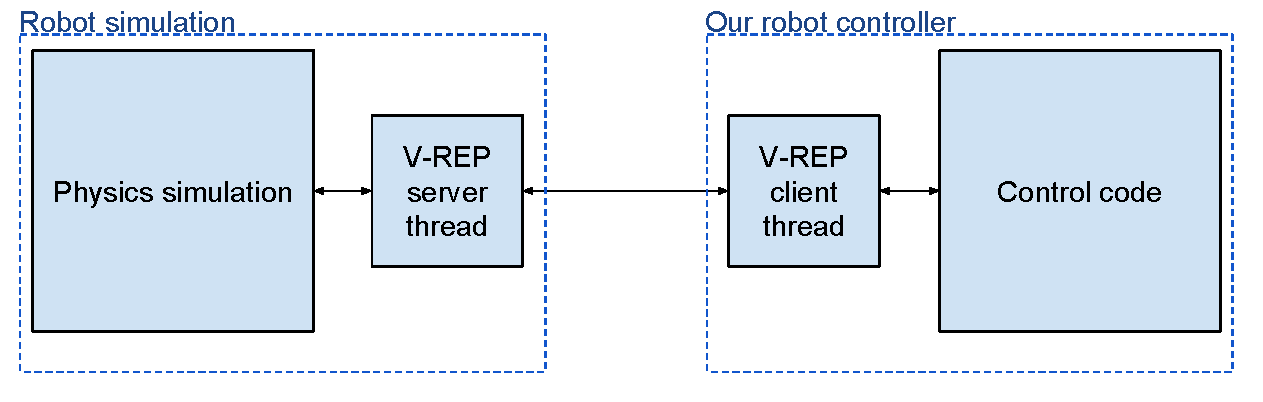
\includegraphics[width=0.7\textwidth]{figures/simulation_principles}
\caption[Simulation principles]{V-Rep simulates the robot while an external program sends order to the robot over TCP/IP thanks to the client/server thread provided by V-Rep.}
\label{fig:simulation_principles}
\end{figure}

These two components can either be executed synchronously or asynchronously. In synchronous operation mode, V-Rep will execute the simulation loop without interruption while handling the requests from the controller between two consecutive iterations. The controller cannot take too long to compute its orders or the simulation will have moved on and the robot will be in a different state than expected. In a way, this is also true for a real robot controller. We choose to work synchronously: each each simulation timestep must be triggered by the control code, as shown in \Cref{fig:remoteApi}.

\begin{figure}[htp]
\centering
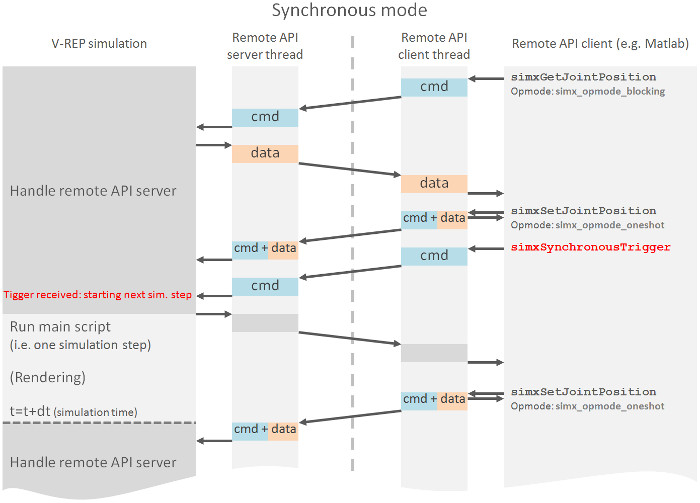
\includegraphics[width=0.8\textwidth]{figures/remoteApiSynchronous}
\caption[Simulation interaction]{Typical interaction between the simulator and the control code. The simulation runs on two threads: the simulation and the server thread. The latter can receive orders from a client thread which is controlled by a custom application of our own. The simulator waits for a trigger before simulating the next timestep. Source: \cite{vrep_manual}}
\label{fig:remoteApi}
\end{figure}

\section{Applications}
This section presents some simulations we made in order to prove the ability of a robot to stand, stand up or move from one lying position to another. The model we use is the one presented at the end of the previous chapter, shown in \cref{fig:robotv7}.

\subsection{Static stability}
The first application is a simple test of the robot's ability to stand upright on its own, using the servomotors. The servomotors of the robot are simply ordered to hold their initial angle and the simulation determines that the robot can indeed stand upright without any elaborate control. This is a simple test that can rule out bad designs quite easily and more specifically designs in which the servomotors are not powerful enough.

\subsection{Going from a supine to a prone position}
The main motivation for a routine that makes the robot move from a supine\footnote{lying on the back}  position to a prone\footnote{lying on the belly} one is that it allows us to only have one standing up routine. 

The routine is defined as follows:\begin{enumerate}
\item From $0$ to $0.39sec$: the robot brings his right arm above his head while preparing the left one to lift its body from the left side. Both legs are twisted towards the right side at the hips.

\item From $0.40$ to $0.99sec$: the left leg swings towards the right side while the right leg swings towards the left side. The left elbow prepares to push.

\item From $1.00$ to $1.59sec$: the left elbow pushes the body up and the hips untwist. The left feet touches the ground on the right side.

\item At $1.6sec$: The robot relaxes all its limbs and is now prone.
\end{enumerate}

The evolution of the angles held by the joints during the routine is presented in \cref{fig:sup2proneArms} and \cref{fig:sup2proneLegs}. The control code is in \Cref{code:go_prone} of the appendices.

\begin{figure}[htp]
\centering
    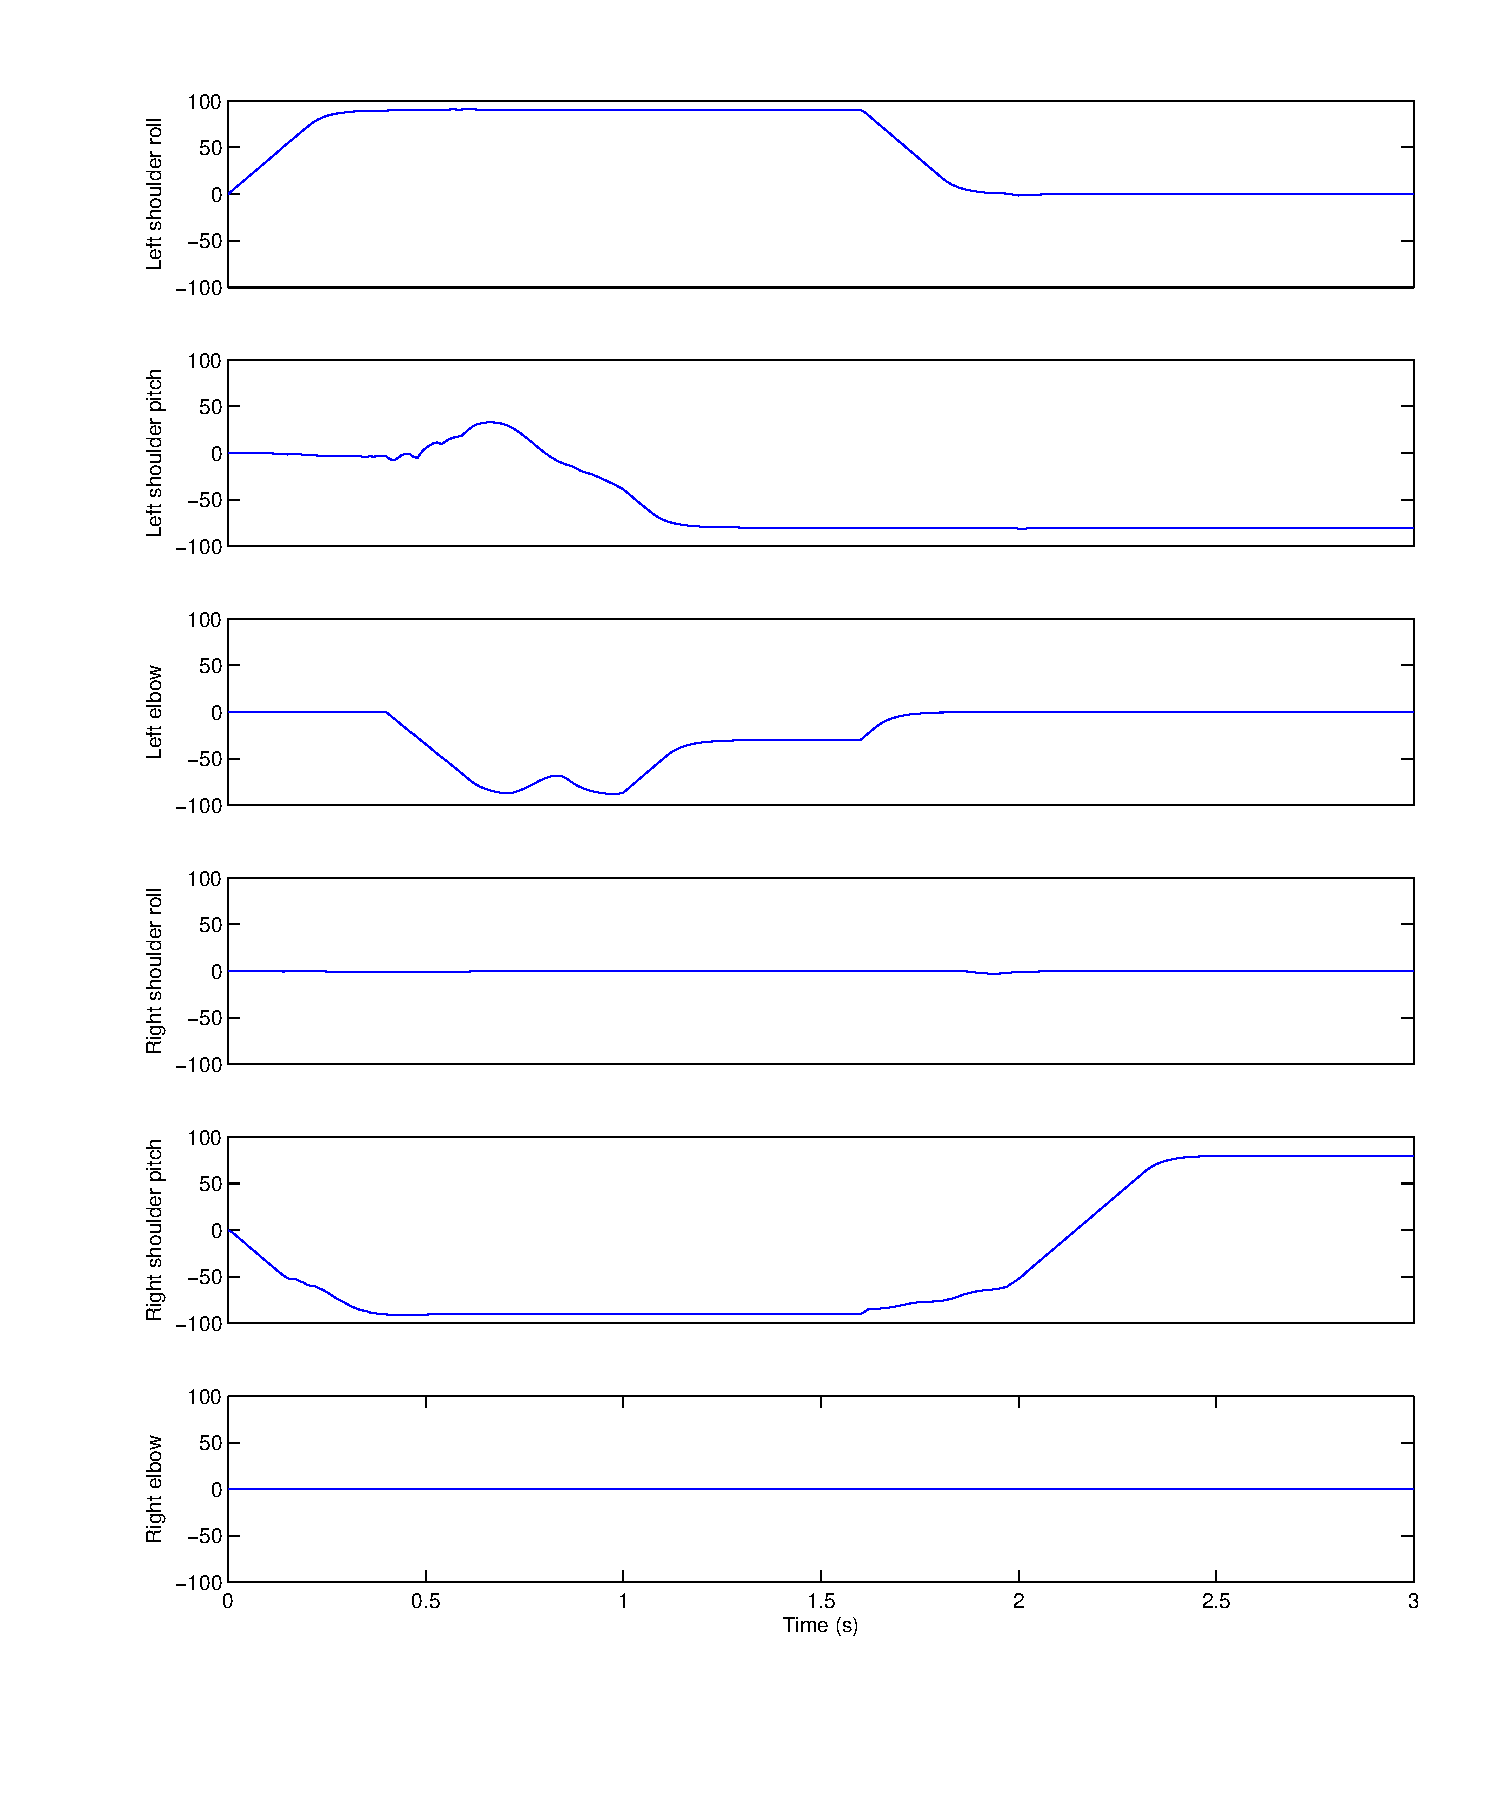
\includegraphics[width = \textwidth]{figures/sup2proneArms}
    \caption[Angles of the arms during \emph{supine} to prone manoeuvre]{Angles of the arms during \emph{supine to prone} manoeuvre. Predictably it is the left arm that is the most active as it is the one that is used to make the robot roll over. We notice that at times (around $0.7sec$) the left elbow does not generate enough torque to hold the desired angle.}
    \label{fig:sup2proneArms}
\end{figure}

\begin{figure}[htp]
\centering
    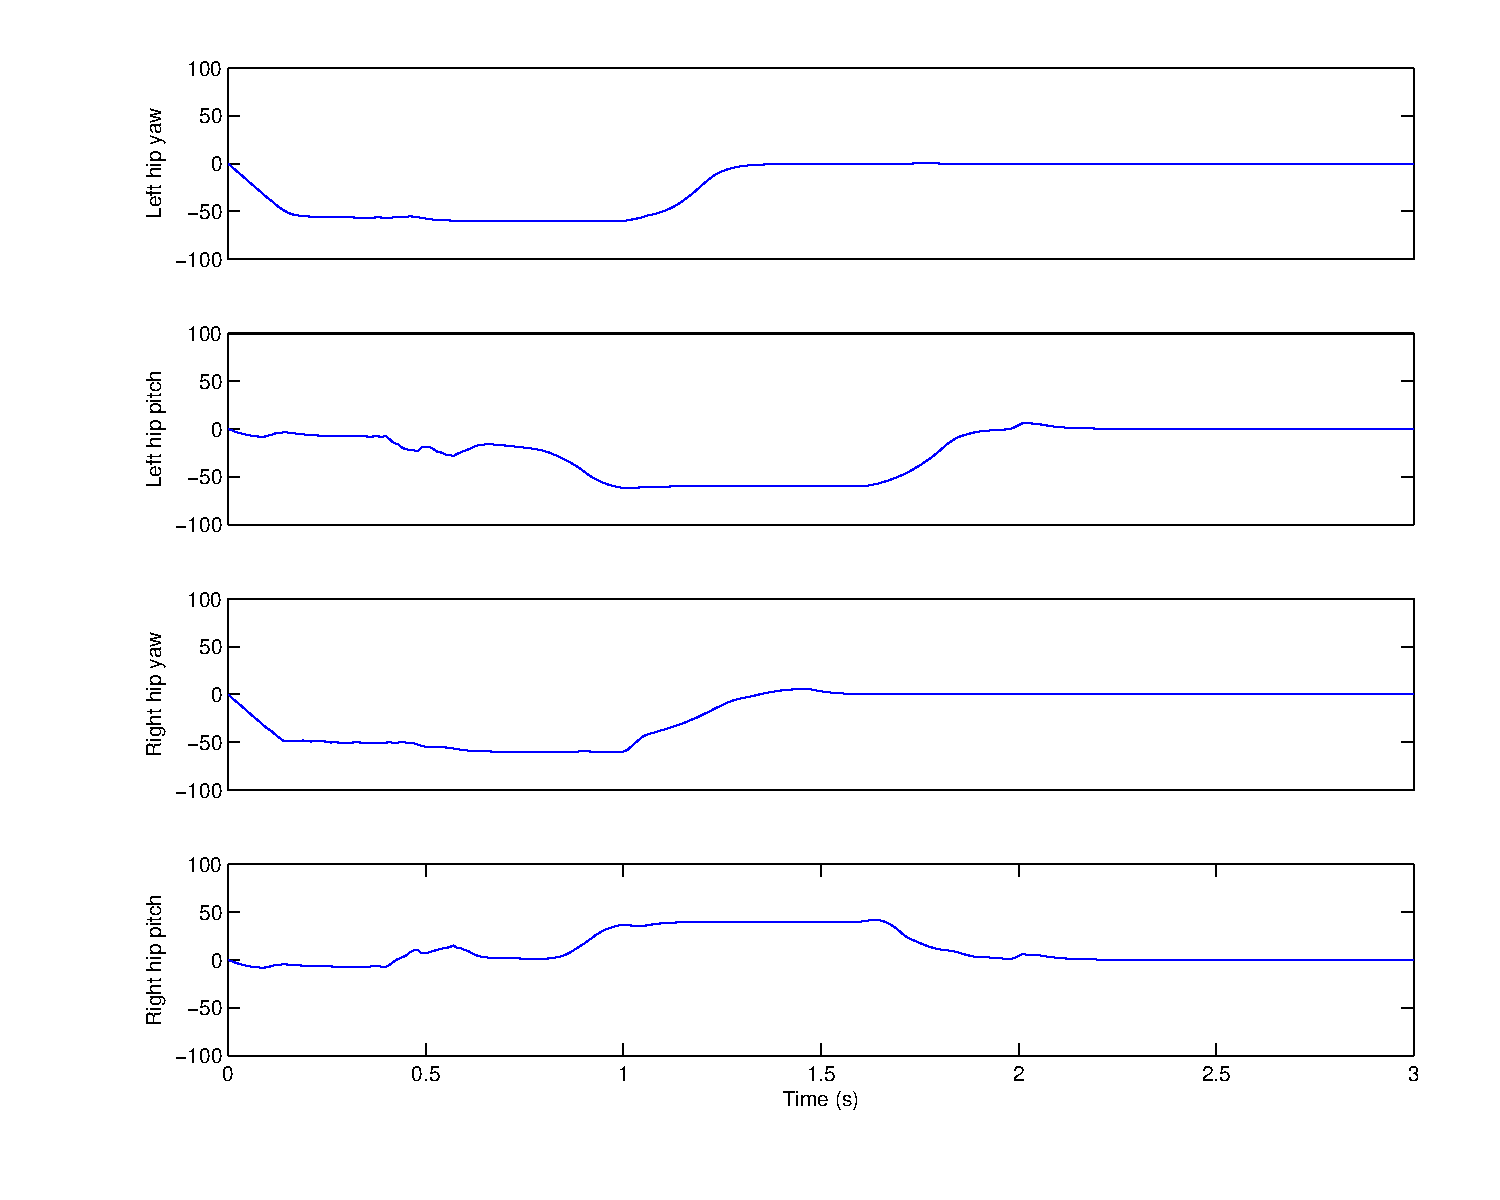
\includegraphics[width = \textwidth]{figures/sup2proneLegs}
    \caption[Angles of the legs during \emph{supine to prone} manoeuvre]{Angles of the legs during \emph{supine to prone} manoeuvre. Both hips are twistes towards the right side but the legs go in opposite directions, the left one towards the right side and the right one towards the left side. Similarly to the previous figure, we notice that sometimes the servomotors cannot hold the desired angle.}
    \label{fig:sup2proneLegs}
\end{figure}

\clearpage
\subsection{Standing up from a prone position}
This routine was inspired by Jörg Stückler, Johannes Schwenk, and Sven Behnke in \cite{Stuckler06}. It is defined as follows:\begin{enumerate}
\item From $0.00$ to $0.19sec$: in preparation for the arms to lift the body in the next step we adjust the roll of the shoulders.

\item From $0.20$ to $0.49sec$: in order to reduce the stress on the servos of the arm, we bend the arms a little before the next step.

\item From $0.50$ to $0.89sec$: lift the body up through the hips with the help of the arms. This step and the next are preparation for the next step where we will move the feet underneath the body.

\item From $0.90$ to $1.39sec$: now that the body is held up by the arms we reverse the holding angle for the hips, to move the hips up. 

\item From $1.40$ to $1.99sec$:  we move the feet underneath the body by bending the knees and bringing the legs closer to the body. The objective is to bring the COM inside the support area of the feet.

\item From $2.80$ to $4.00sec$: the robot slowly gets up by unbending the knees and the hips. 
\end{enumerate}

The evolution of the angles held by the joints during the routine is presented in \cref{fig:prone2standArms} and \cref{fig:prone2standLegs}. The control code is in \Cref{code:stand_prone} of the appendices.

\begin{figure}[htp]
\centering
    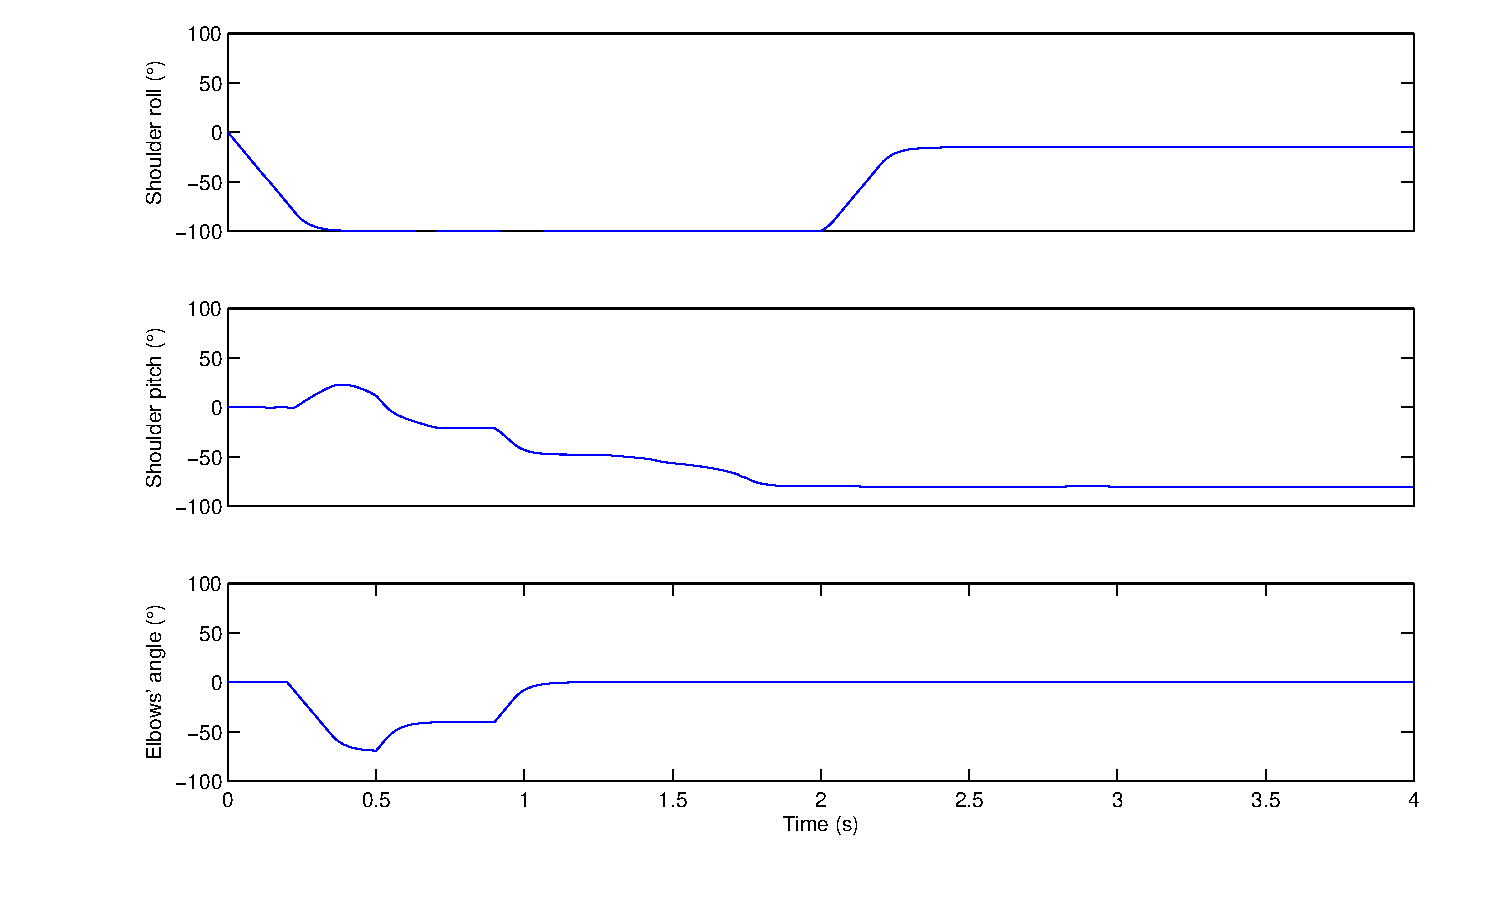
\includegraphics[width = \textwidth]{figures/prone2standArms}
    \caption[Angles of the arms during \emph{supine} to prone manoeuvre]{Angles of the arms during \emph{supine to prone} manoeuvre. Contrary to last time both arms receive the same orders. At first, the servomotors in the shoulders rotate the arms to put them in the right position for pushing. The elbows are bent to help the servos in the shoulders lift the trunk.}
    \label{fig:prone2standArms}
\end{figure}

\begin{figure}[htp]
\centering
    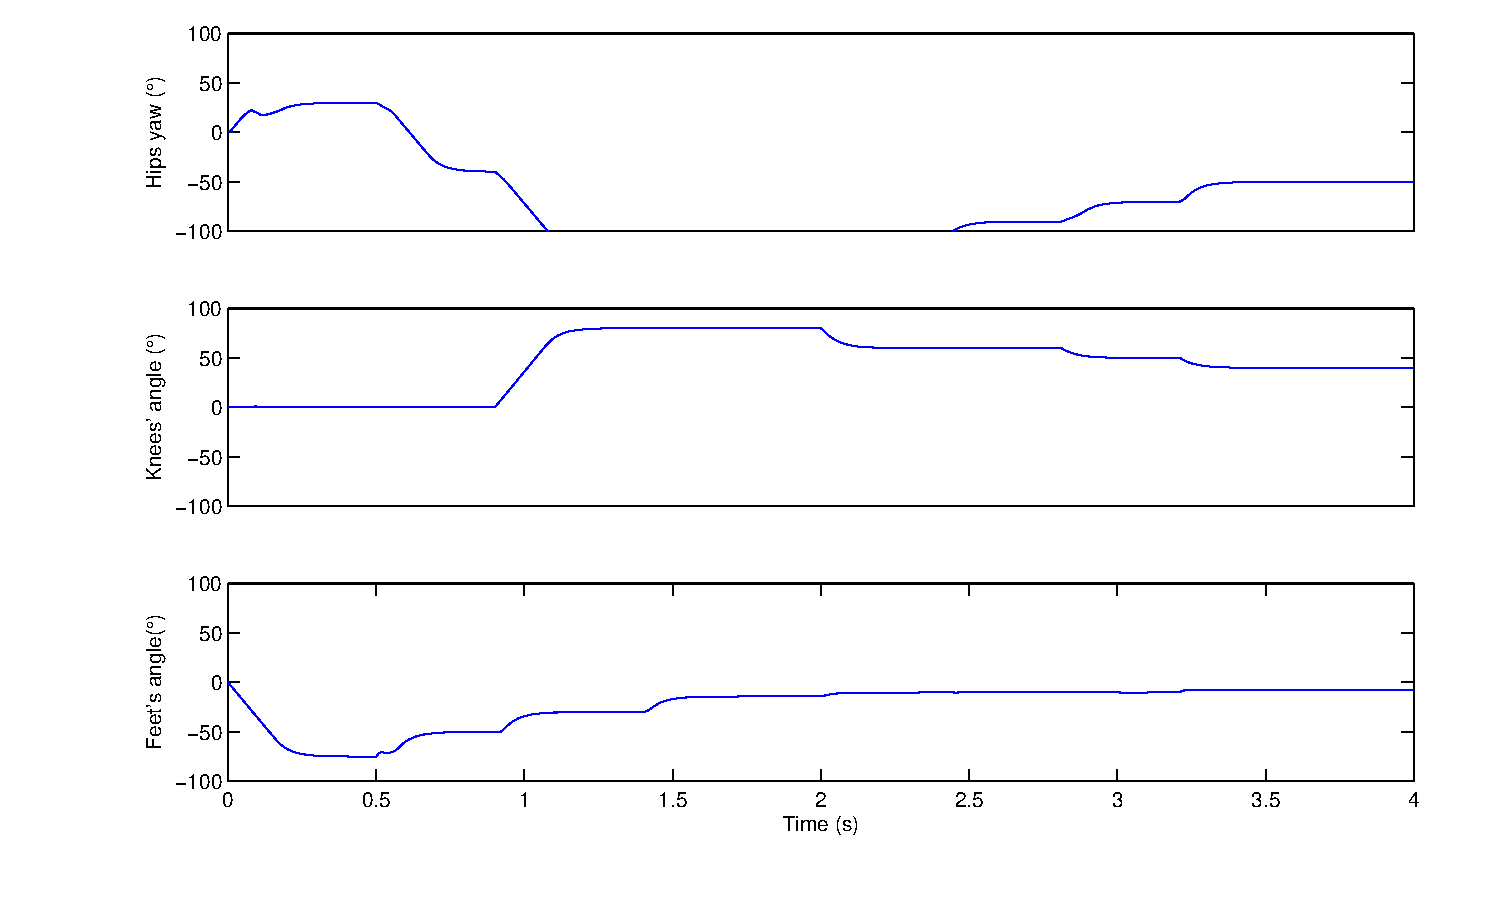
\includegraphics[width = \textwidth]{figures/prone2standLegs}
    \caption[Angles of the legs during \emph{supine to prone} manoeuvre]{Angles of the legs during \emph{supine to prone} manoeuvre. Again, both legs receive the same orders. Notice the importance of footwork in this routine.}
    \label{fig:prone2standLegs}
\end{figure}

\section{Influence of the simulations on the design of the robot}

\begin{figure}[htp]
	\centering
	\begin{subfigure}[b]{0.48\textwidth}
		\centering
		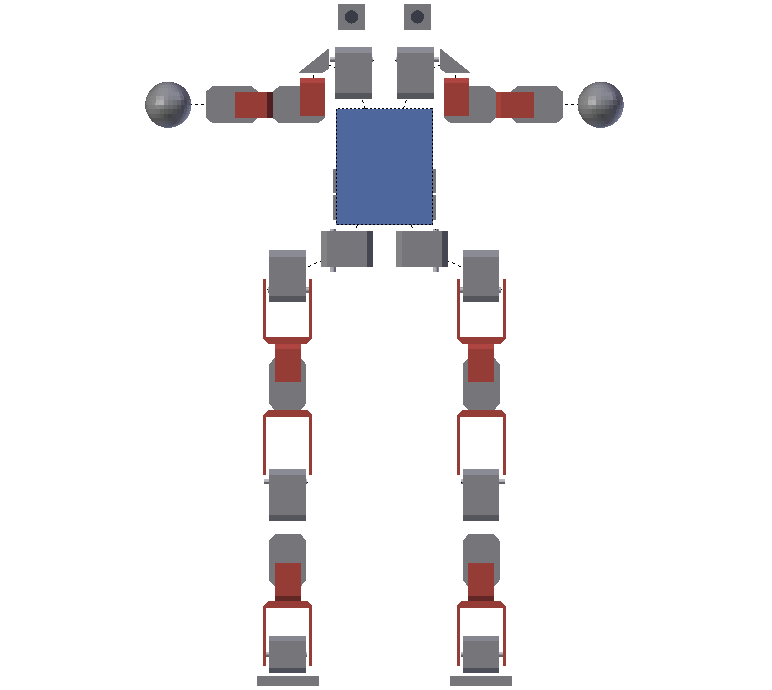
\includegraphics[width = 0.84\textwidth]{figures/robot_v2}
		\caption{1st iteration. \label{fig:robot_v2}}
	\end{subfigure}
	\hfill
	\begin{subfigure}[b]{0.48\textwidth}
		\centering
		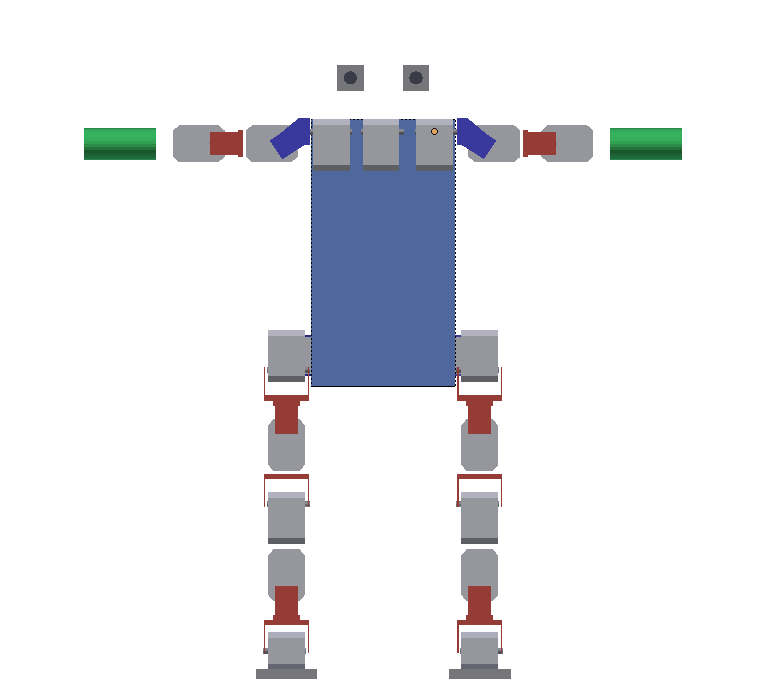
\includegraphics[width = 0.84\textwidth]{figures/robot_v3}
		\caption{2nd iteration. \label{fig:robot_v3}}
	\end{subfigure}
	
	\begin{subfigure}[b]{0.48\textwidth}
		\centering
		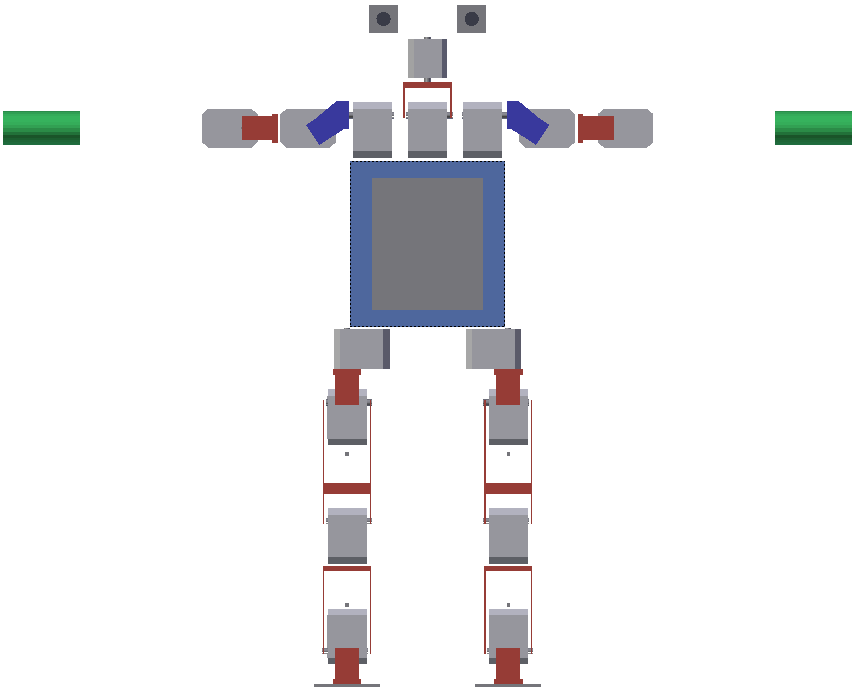
\includegraphics[width = \textwidth]{figures/robot_v5}
		\caption{3rd iteration. \label{fig:robot_v5}}
	\end{subfigure}
	\hfill
	\begin{subfigure}[b]{0.48\textwidth}
		\centering
		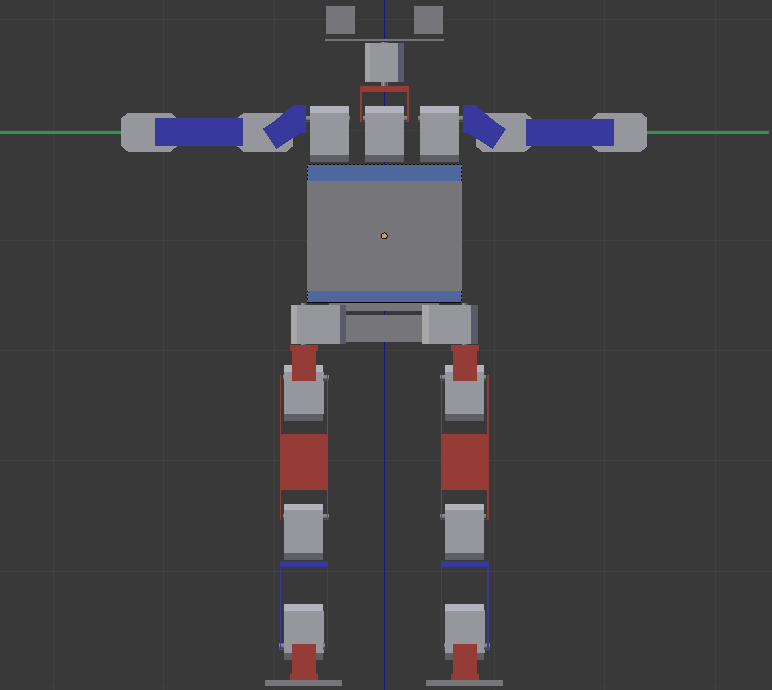
\includegraphics[width = 0.84\textwidth]{figures/robot_v7_front}
		\caption{Final and last iteration. \label{fig:robot_v7}}
	\end{subfigure}
	\caption[Evolution of the robot design]{Evolution of the robot design.}
	\label{fig:evolution}
\end{figure}

The ultimate purpose of this work was to help the team of students design a humanoid robot able of participating in RoboCup contest. This section highlights the main influences our work had on the design of the robot.

The first robot we tried to simulate was the one in \Cref{fig:robot_v2}. At that time, it was not clear if the cameras at the top were to be moved by MX-28R servomotors or some smaller and cheaper servos hence the absence of servos under them. The hands (the balls) were still in their early phase and were approximated by balls, the main idea being that some sort of element is needed between the last servo of the arm and ground. The legs were very long as the servos were all the same plane. This design has never been thoroughly tested, it was more of an exercise. It was too inaccurate for the simulations to be of any use. We show it here for the purpose of presenting the design ideas that existed at the beginning of the project.

The first robot we really tested is the one in \Cref{fig:robot_v3}. A third servo has appeared at the top of the robot and the hands became cylinders. The legs are shorter, because the servos that connect the legs to the trunk are now hidden behind the trunk. Which got longer and larger. This robot did not perform very well. Its arms were too short for it to be able to stand up. The range of movements of its joints was also too limited, especially at the feet, knees and hips. 

The third iteration (\Cref{fig:robot_v5}) tried to overcome these limitations. The arms are longer and the legs were modified to have a wider movement range (some servos were connected together, in the fashion that is visible in \Cref{fig:robotv7_side}). After some adjustments of the length of the hinges in the legs it was able to stand up but by making the servos in the arms stronger than the MX-28R really is. It was this model that had collision problems we mentioned in \Cref{sec:modelling} because its feet were too thin. 

The last design (\Cref{fig:robot_v7}) thus has different arms from its predecessor. The servos at their extremities are placed in the middle. The hands became rectangular plates. The batteries are also placed lower in an effort to lower the centre of mass. This design, as you already know, was able to stand up and perform other routines. It also respect the rules of the contest (see \cref{appendix:rules}):
\begin{enumerate}
	\item Height ($H_{top}$):  $40 \leq 61.75 \leq 90cm$.
	\item Weight: $2.726kg$.
	\item Height of centre of mass ($H_{COM}$): $34cm$. Foot area: $175 < cm^2$.
	\item Foot aspect ratio: $1.79 \leq 2.5$.
	\item Minimal width of the robot: $20 \leq 33.96cm$.
	\item $69.72 \leq 74.10cm$.
	\item Maximal height: $75.52 < 92.63cm$.
	\item Leg length ($H_{leg}$): $21.61 \leq 27.5 \leq 43.23cm$.
	\item Height of the head ($H_{Head}$): $3.09 \leq 10.75 \leq 15.44cm$.
\end{enumerate}
